% -------------------------------------------------------------
% Template HOMEWORK
% -------------------------------------------------------------
% 2020 by d!egofantinelli at jazzmagus@gmail.com
% -------------------------------------------------------------

% ---------------------------------- Preambolo
\documentclass[12pt, a4paper, landscape]{exam}
\usepackage[T1]{fontenc}
\usepackage{mdframed}
%\usepackage{nicefrac}
%\usepackage[applemac]{inputenc}
%\usepackage[utf8]{inputenc}
\usepackage[export]{adjustbox}
\usepackage[italian]{babel}
\usepackage[margin=1in]{geometry}
\usepackage{amsfonts, amsthm, amsmath, amssymb}
\usepackage{multicol}
\usepackage{mathrsfs}
\usepackage[none]{hyphenat}
\usepackage{bbm}
\usepackage{graphicx}
\usepackage{tikz}
%\usepackage[dvipsnames]
%\usepackage{upquote}
\usepackage{caption}
\usepackage{float}

%\printanswers

% ---------------------------------- General Math Setup
\newcommand{\numberset}{\mathbb}
\newcommand{\N}{\numberset{N}}
\newcommand{\Z}{\numberset{Z}}
\newcommand{\Q}{\numberset{Q}}
\newcommand{\R}{\numberset{R}}

\newcommand{\ChoiceLabel}[1]{\hspace{-1.6em}\makebox[1.6em][l]{\textbf{#1.}}\ignorespaces}

\newcommand{\WrongChoice}[1]{\choice \ChoiceLabel{#1}}
\newcommand{\RightChoice}[1]{\correctchoice \ChoiceLabel{#1}}
\newcommand{\Item}[1]{\hspace{-17pt}\makebox[17pt][l]{\textbf{#1.}}\ignorespaces}

\renewcommand{\solutiontitle}{\noindent\textbf{Soluzione:}\par\noindent}

\renewcommand{\questionshook}{%
    \setlength{\leftmargin}{0pt}%
}
\renewcommand{\choiceshook}{%
    \setlength{\leftmargin}{20pt}%
}

% ---------------------------------- Intestazione
\newcommand{\class}{\LARGE {Esercizio: Studio di Funzione reale di variabile reale}}
%%\newcommand{\term}{I Quadrimestre}
%\newcommand{\examnum}{Verifica numero: 1}
%\newcommand{\examdate}{11 dicembre 2020}
%\newcommand{\timelimit}{40 minuti}
\CorrectChoiceEmphasis{\color{red}}
\SolutionEmphasis{\color{red} \footnotesize}
\renewcommand{\solutiontitle}{\noindent\textbf{Soluzione:}\par\noindent}


% ---------------------------------- Intestazione
\pagestyle{headandfoot}
\footrule
\headrule
\lhead{MATEMATICA}
\rhead{Classe 5\string^QA}
\chead{IIS "G. A. Remondini" - Bassano del Grappa (VI)}
\rfoot{25 marzo 2021}
\lfoot{Pag. \thepage\ of \numpages}

% ---------------------------------- Punteggi
%\pointpoints{punto}{\em punti}
%\pointformat{[{\footnotesize \thepoints}]}
%\bonuspointpoints{punto bonus}{\em punti bonus}
%\bonuspointformat{[{\footnotesize \thepoints}]}
%\pointsinrightmargin
%\setlength{\rightpointsmargin}{.2cm}
%\chqword{Esercizio}
%\chpword{Punti}
%\chbpword{Punti Bonus}
%\chsword{Punteggio}
%\chtword{Totale}

\begin{document}

% ---------------------------------- Title Page
%\vspace{2cm}

{\huge{\bf \class}}\\

{\Large{Seguendo la traccia indicata, studia la funzione seguente, e ipotizza un grafico plausibile}}:\\

{\large {\(y = f(x) = \dfrac {x^2 - x^3}{x^2 + 3}\)}}\\

% ====================== VERIFICA 

\begin{questions}

\begin{multicols}{2}
% ------------------------------------------- Esercizio #1
%\addpoints
\question
Insieme di Definizione:
\fillwithdottedlines{0.5in}
\vspace{0.3cm}

% ------------------------------------------- Esercizio #2
\question
Eventuali Intersezioni con gli Assi di Simmetria:

\fillwithdottedlines{0.5in}
\vspace{0.2cm}

\question Eventuali simmetrie:
\fillwithdottedlines{0.5in}
\vspace{0.2cm}

\question Studio del Segno: \(f(x) \ge 0\):
\fillwithdottedlines{0.5in}
\vspace{0.2cm}
\question Limiti agli estremi dell'Insieme di Definizione:

\fillwithdottedlines{0.5in}
\vspace{0.2cm}

\question Grafico {\em ipotetico}: \(f(x) \ge 0\):\\

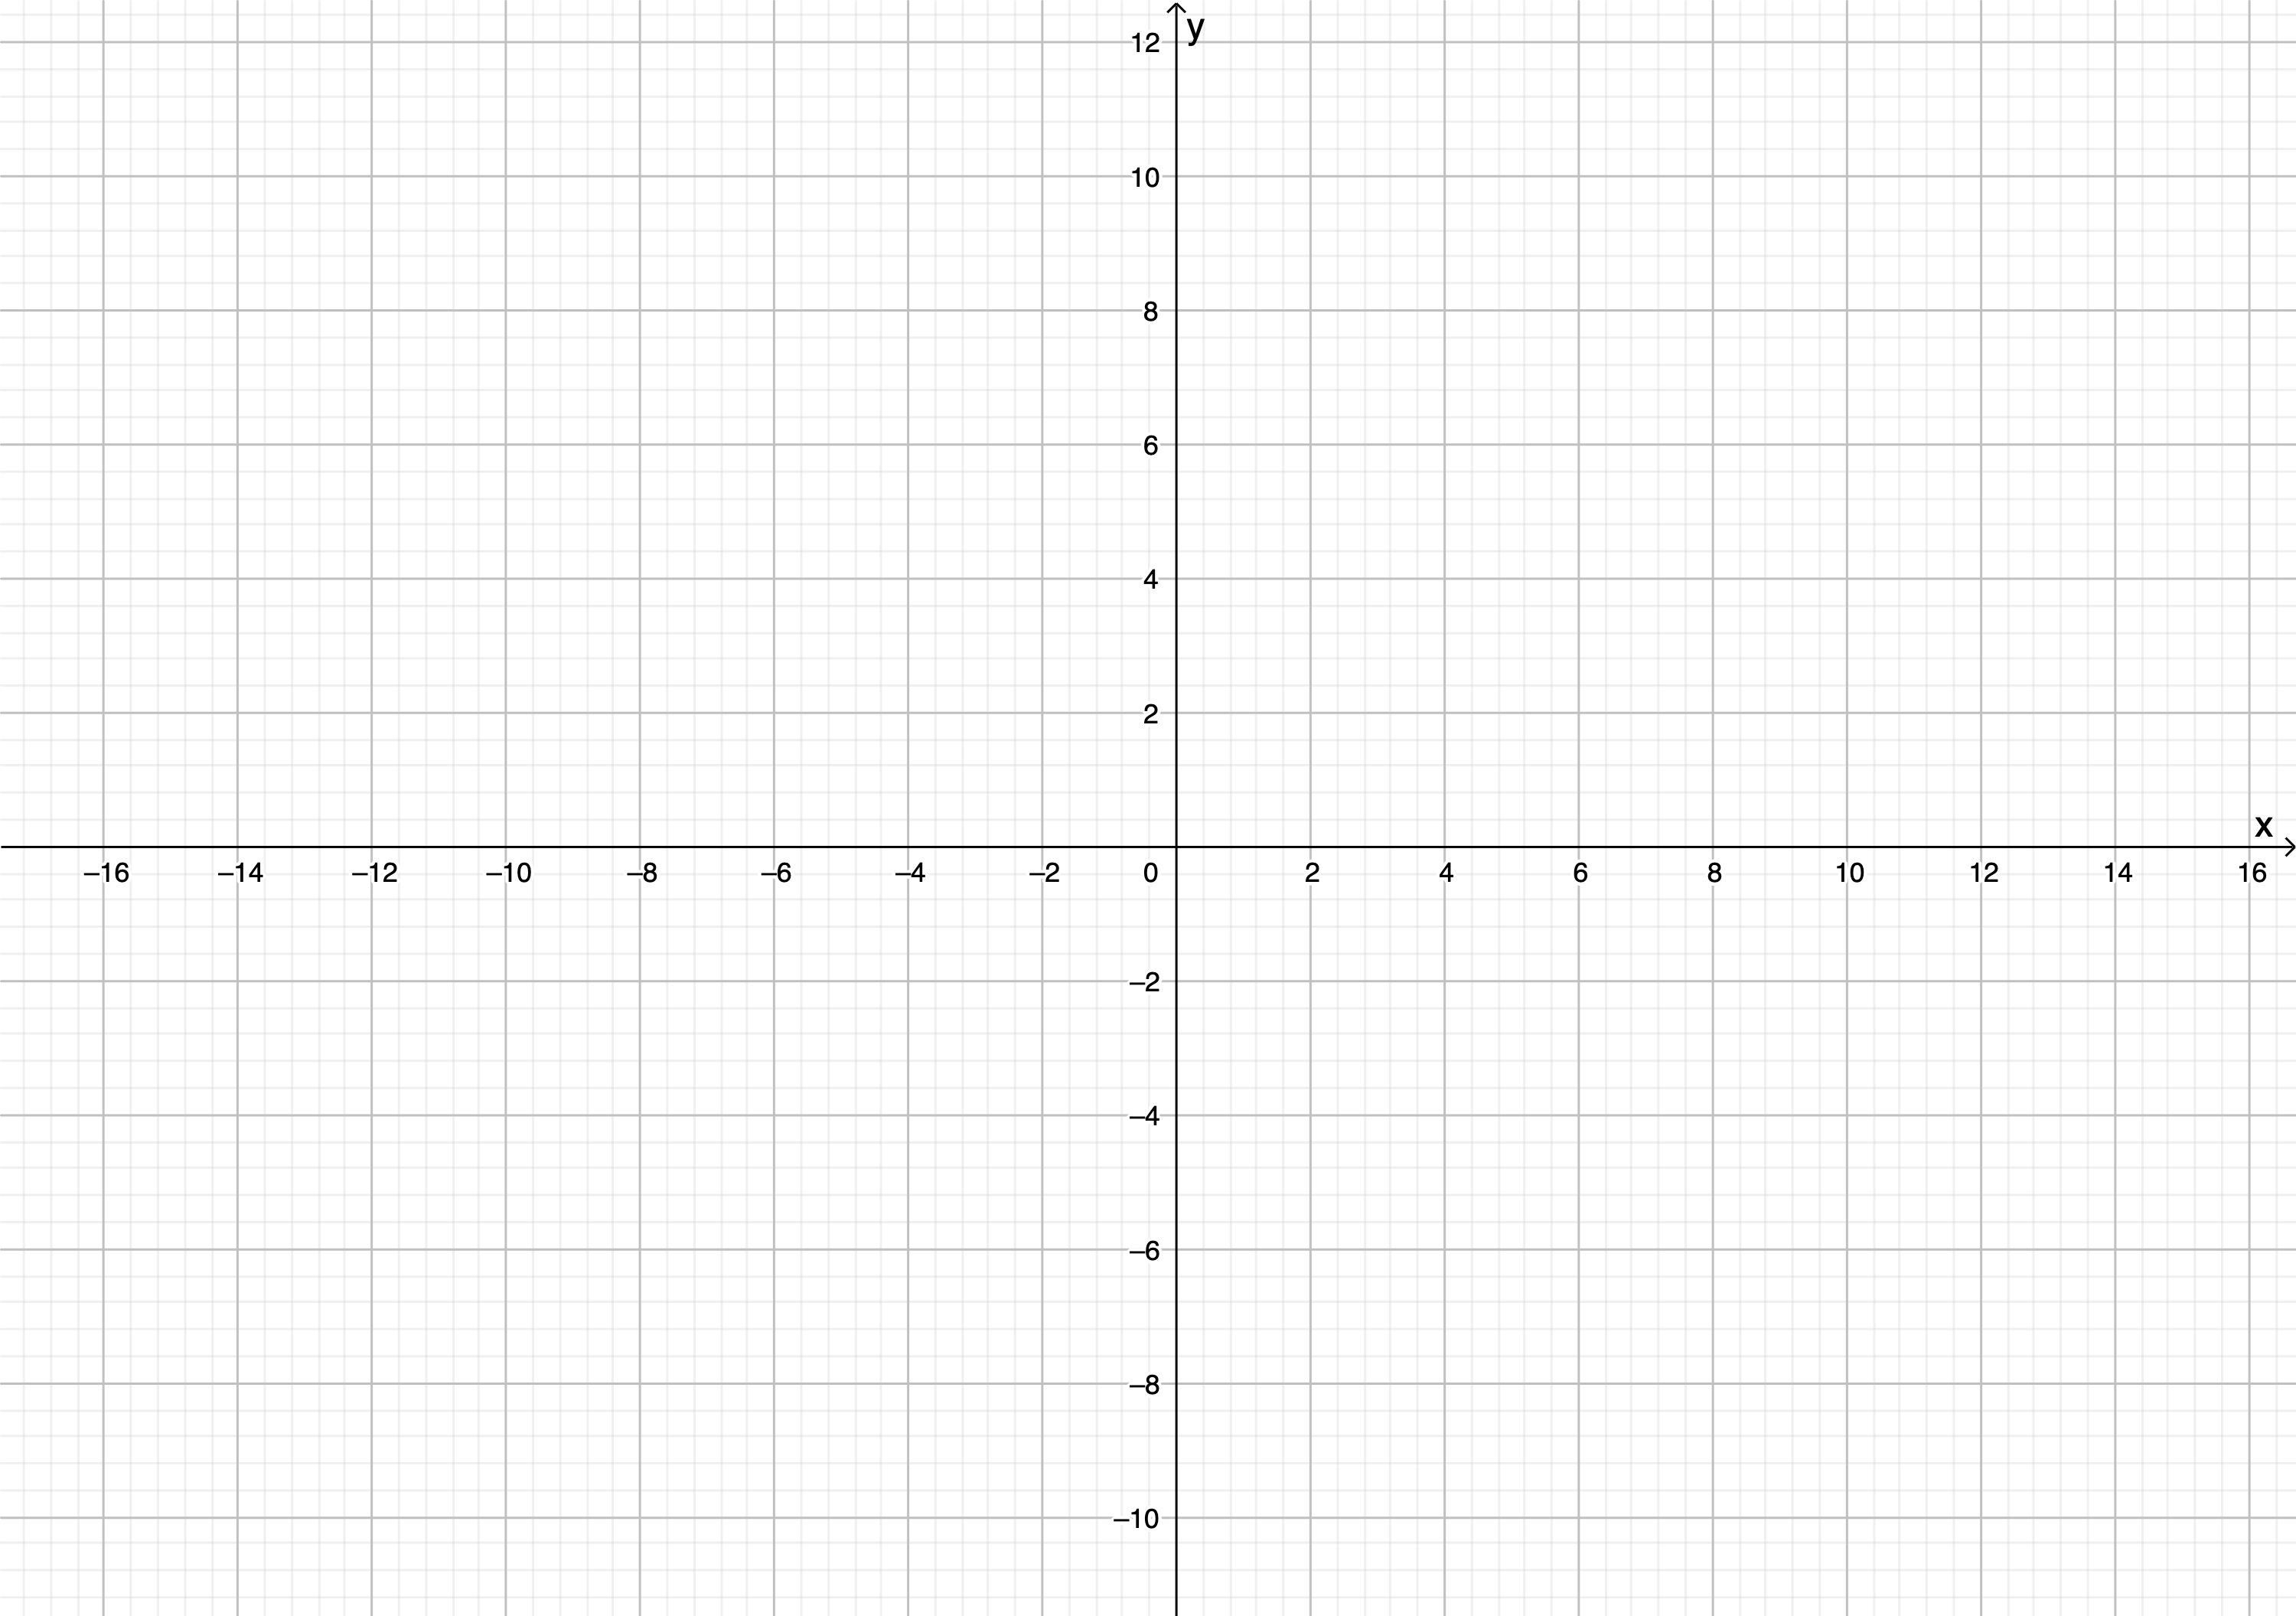
\includegraphics[width=\columnwidth, fbox]{grafico_empty.png}

%\begin{tikzpicture}
%\draw[help lines, color=gray!50, dashed] (-4.9,-4.9) grid (4.9,4.9);
%\draw[->,thick] (-6,0)--(6,0) node[below]{$x$};
%\draw[->,thick] (0,-5.5)--(0,5.5) node[left]{$y$};
%
%\end{tikzpicture}

\end{multicols}
\end{questions}
%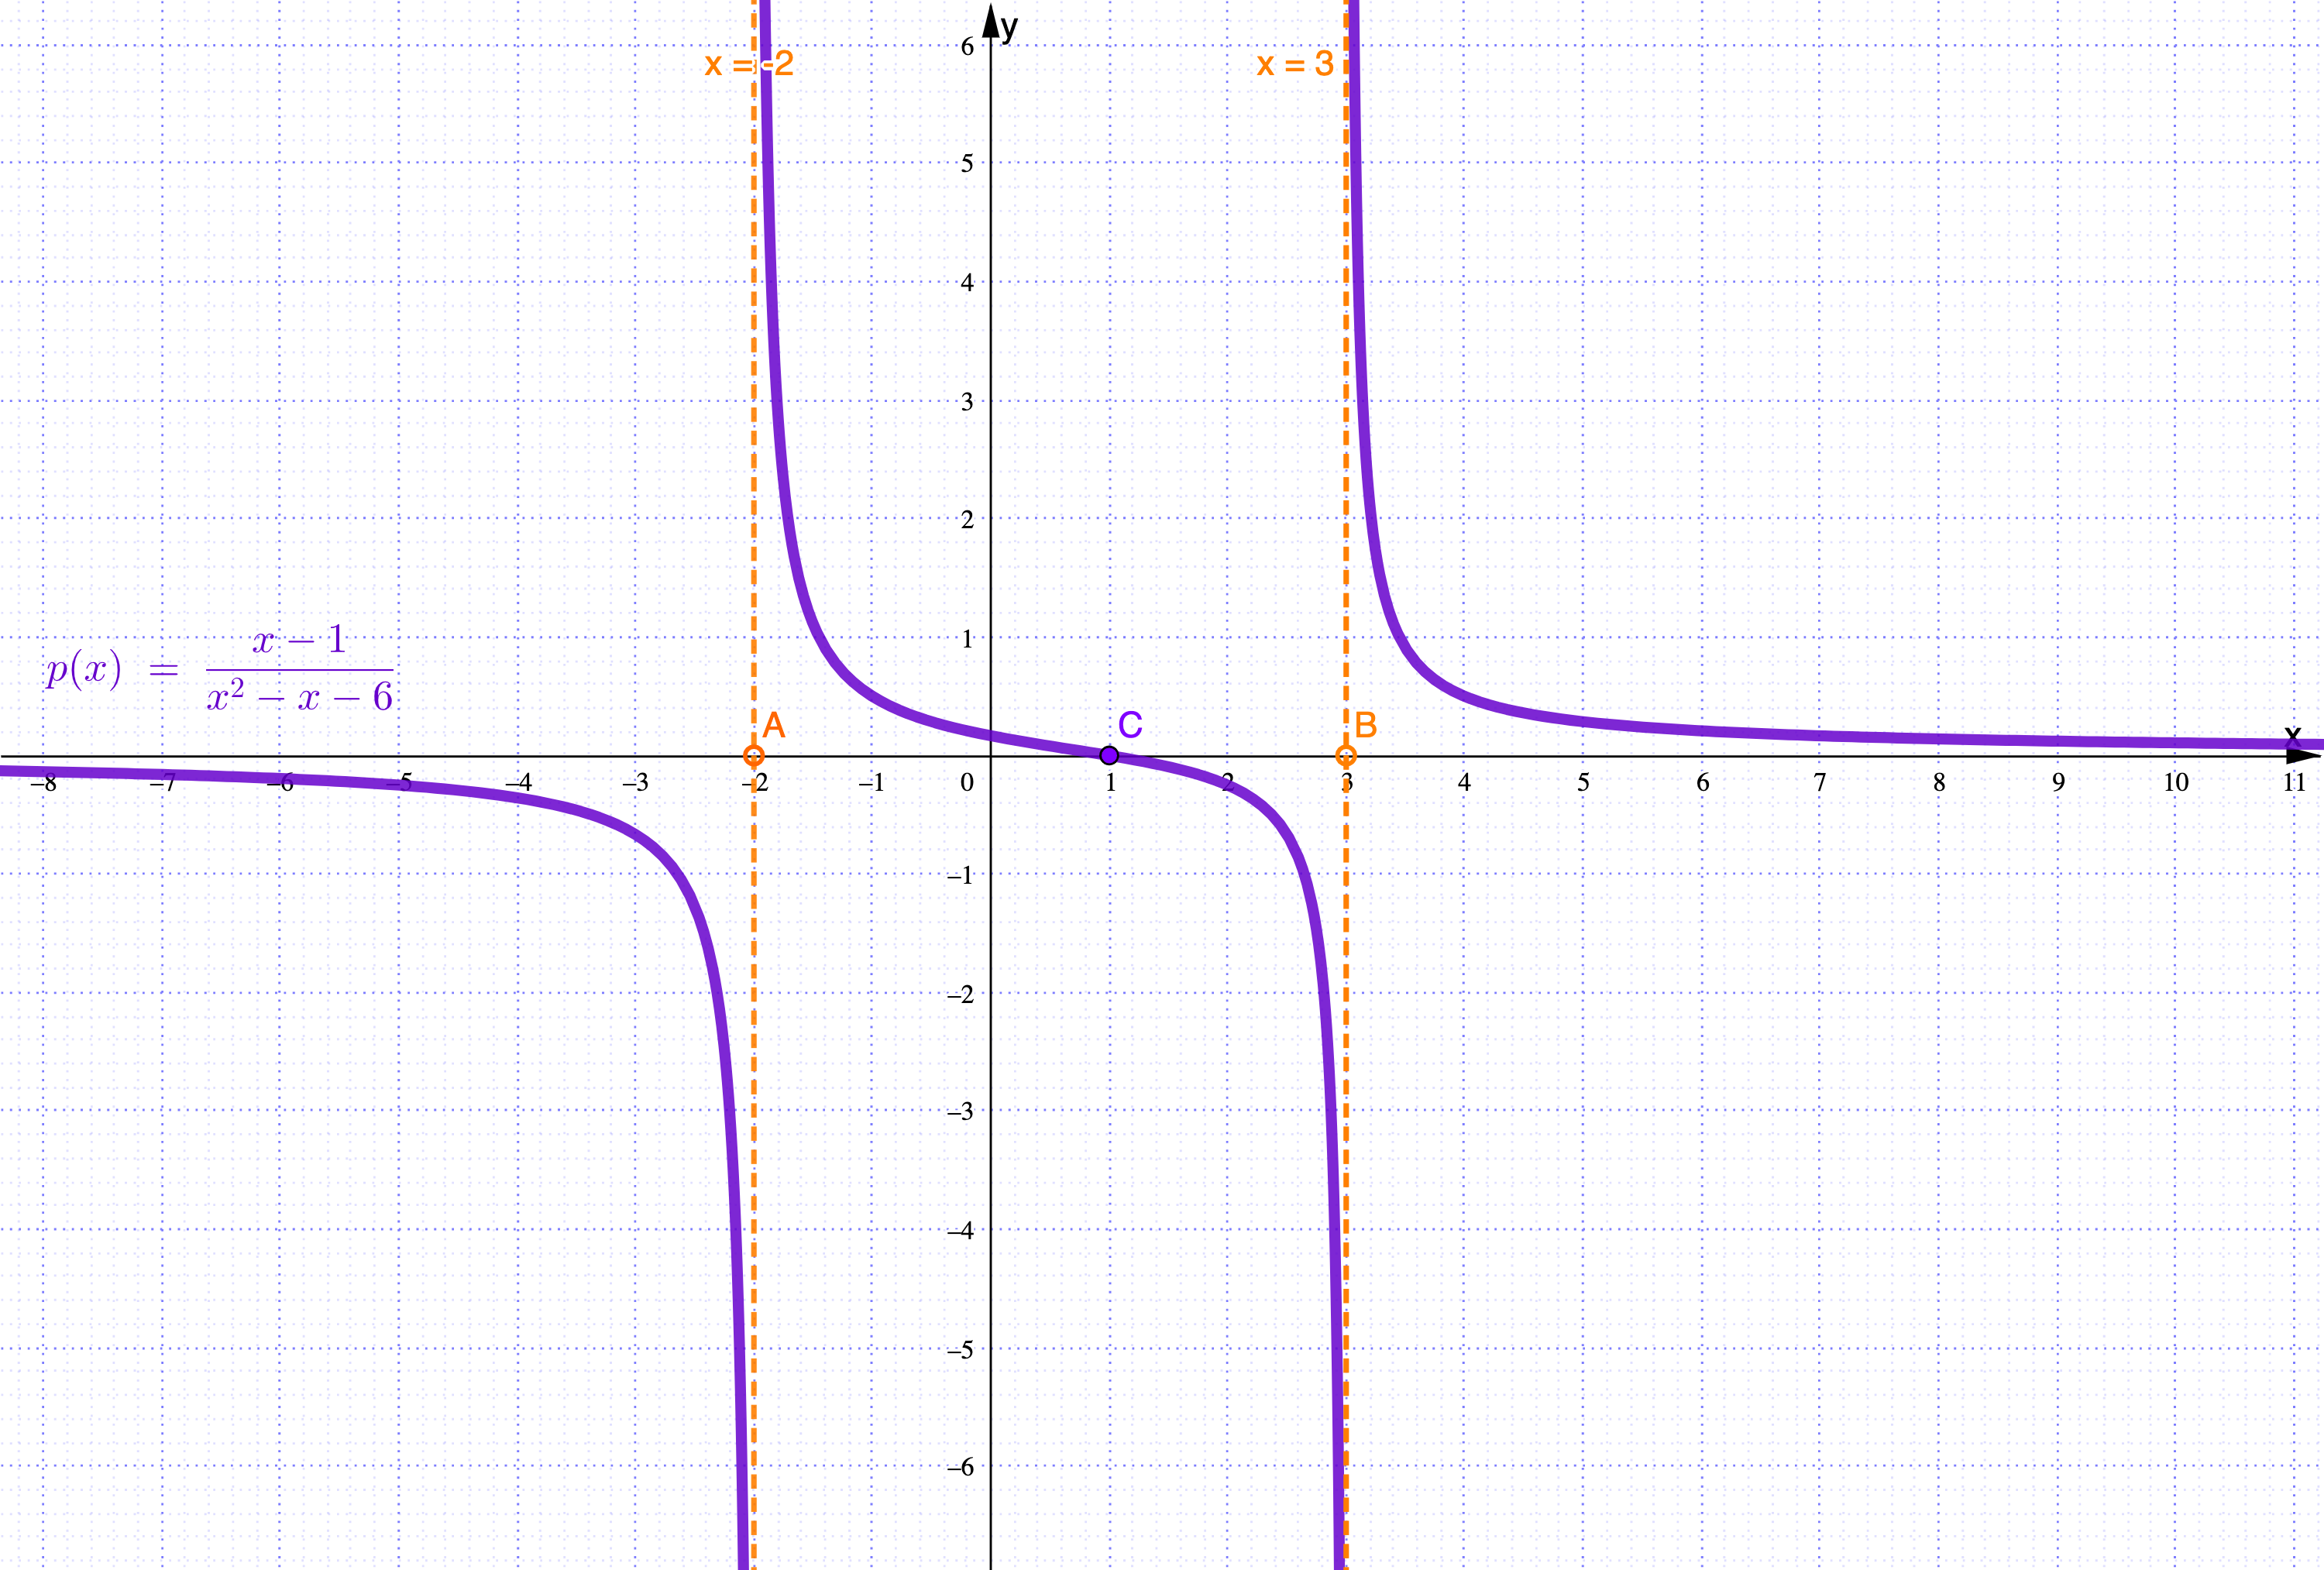
\includegraphics{hw_graph_01}

\end{document}
